\chapter{Problematyka zagadnienia}
\label{ch:problematyka}

\section{Charakterystyka choroby Parkinsona}
\label{sec:charakterystykaPD}


Choroba Parkinsona (PD) jest zwyrodnieniowym schorzeniem mózgu związanym z objawami motorycznymi (spowolnienie ruchowe,
drżenie, sztywność, zaburzenia chodu i równowagi) oraz szeroką gamą powikłań niemotorycznych (zaburzenia poznawcze,
zaburzenia psychiczne, zaburzenia snu oraz ból i inne zaburzenia sensoryczne).
Objawy zwykle zaczynają się stopniowo i nasilają z czasem.
Ich postęp powoduje wysoki stopień niepełnosprawności i konieczność opieki.
U wielu osób z PD w trakcie trwania choroby mogą również rozwinąć się zmiany psychiczne i behawioralne, problemy ze snem,
depresja, problemy z pamięcią i zmęczenie.

Chociaż każdy może być narażony na ryzyko rozwoju choroby Parkinsona, badania naukowe sugerują,
że choroba ta dotyka więcej mężczyzn niż kobiet.
Statystyki pokazują, że ryzyko zachorowania rośnie wraz z wiekiem, chociaż choroba może dotyczyć także młodszych osób.
U większości osób z PD po raz pierwszy choroba rozwija się po 60 roku życia, około 5\% do 10\% doświadcza jej początku przed 50 rokiem życia.
Postacie choroby Parkinsona o wczesnym początku są często, choć nie zawsze, dziedziczne i niektóre formy zostały powiązane z
określonymi zmianami w genach\cite{National_Institute_on_Aging_2022}.


Najbardziej widoczne oznaki i objawy choroby Parkinsona pojawiają się, gdy komórki nerwowe w zwojach podstawy mózgu,
obszarze mózgu kontrolującym ruch, ulegają uszkodzeniu i/lub obumierają.
Zwykle te komórki nerwowe lub neurony wytwarzają dopaminę.
Kiedy neurony obumierają lub ulegają uszkodzeniu, wytwarzają mniej dopaminy, co powoduje problemy z poruszaniem się
związane z chorobą.
Na ten moment nie wiadomo co powoduje śmierć neuronów.
Zanikają również zakończenia nerwowe, które wytwarzają norepinefrynę, główny przekaźnik chemiczny
współczulnego układu nerwowego, który kontroluje wiele funkcji organizmu, takich jak tętno i ciśnienie krwi.
Utrata norepinefryny może pomóc wyjaśnić niektóre cechy choroby Parkinsona związane z brakiem ruchu, takie jak zmęczenie,
nieregularne ciśnienie krwi, zmniejszony ruch pokarmu w przewodzie pokarmowym i nagły spadek ciśnienia krwi, gdy osoba wstaje z pozycji siedzącej lub leżącej.


Przyczyna PD nie jest znana, ale uważa się, że powstaje w wyniku złożonej interakcji pomiędzy czynnikami genetycznymi i
narażeniem na czynniki środowiskowe, takie jak pestycydy, rozpuszczalniki i zanieczyszczenia powietrza.
Niektóre przypadki PD wydają się być dziedziczne, a kilka przypadków można przypisać określonym wariantom genetycznym.
Chociaż uważa się, że genetyka odgrywa rolę w chorobie Parkinsona, w większości przypadków choroba nie występuje rodzinnie\cite{National_Institute_on_Aging_2022}.

Choroba Parkinsona ma cztery główne objawy:
\begin{itemize}
\item Drżenie rąk, ramion, nóg, szczęki lub głowy
\item Sztywność mięśni, gdy mięśnie pozostają skurczone przez długi czas
\item Powolność ruchu
\item Zaburzenia równowagi i koordynacji, czasami prowadzące do upadków
\end{itemize}


Pozostałe objawy mogą obejmować:
\begin{itemize}
\item Depresja i inne zmiany emocjonalne
\item Trudności w połykaniu, żuciu i mówieniu
\item Problemy z układem moczowym lub zaparcia
\item Problemy skórne
\end{itemize}

Objawy choroby Parkinsona i tempo progresji różnią się u poszczególnych osób.
Początkowo są subtelne i pojawiają się stopniowo.
Często zaczynają się po jednej stronie ciała lub nawet w jednej kończynie.
W miarę postępu choroby ostatecznie dotyka ona obu stron, jednak objawy mogą być bardziej nasilone po jednej stronie niż po drugiej.
Wiele osób z chorobą Parkinsona zauważa, że przed wystąpieniem sztywności i drżenia miały problemy ze snem, zaparcia, utratę węchu oraz zespół niespokojnych nóg.
Należy pamiętać, że niektóre z tych objawów mogą również wystąpić podczas normalnego starzenia się\cite{National_Institute_on_Aging_2022}.


Według raportu Światowej Organizacji Zdrowia\cite{WHO} w skali globalnej niepełnosprawność i zgony z powodu PD
rosną szybciej niż w przypadku jakichkolwiek innych zaburzeń neurologicznych.
Częstość występowania PD podwoiła się w ciągu ostatnich 25 lat.
Globalne szacunki w 2019 roku wykazały ponad 8,5 miliona osób z PD.
Obecne szacunki sugerują, że w 2019 roku PD spowodowała 5,8 miliona lat życia z niepełnosprawnością, co
stanowi wzrost o 81\% od 2000 roku, i spowodowała 329 000 zgonów, co stanowi wzrost o ponad 100\% od 2000 roku.


[DODAĆ WYKRES]


W Polsce z chorobą Parkinsona zmaga się około 100 tys. pacjentów, z czego około 20\% jest już w stadium zaawansowanym
według informacji przekazywanych przez Fundację Chorób Mózgu.
Ponadto co roku w naszym kraju wykrywanych jest ok. 8 tys. nowych zachorowań.
Nowe zachorowania nadal skorelowane są z wiekiem, średnia wieku chorych wynosi 60 lat, niestety wzrasta odsetek chorych wśród osób młodych (nawet w wieku 20 lat).


\subsection{Głos w chorobie Parkinsona}
\label{subsec:glospd}

Przeprowadzono badanie akustyczne i percepcyjne cech głosu pacjentów z chorobą Parkinsona w zależności od ciężkości choroby.
Charakterystykę percepcyjną i akustyczną głosu 30 pacjentów z chP we wczesnym stadium i 30 pacjentów z chP w późniejszym
stadium porównano z danymi uzyskanymi od 30 zdrowych osób z grupy kontrolnej.
Nagrania głosowe składały się z przedłużenia samogłoski /a/, śpiewu gamy oraz 1-minutowego monologu.
W porównaniu z grupą kontrolną i wcześniej opublikowanymi danymi normatywnymi, głosy pacjentów z PD zarówno we wczesnym,
jak i późniejszym stadium charakteryzowały się percepcyjnie ograniczoną zmiennością tonu i głośności, oddychaniem,
chropowatością i zmniejszoną głośnością.
Wysokie poziomy tonu modalnego charakteryzowały również głosy mężczyzn zarówno we wczesnych, jak i późniejszych stadiach choroby Parkinsona.
Pod względem akustycznym głosy obu grup pacjentów z ChP wykazywały niższe poziomy średniego natężenia i zmniejszone maksymalne
zakresy częstotliwości fonacyjnej w porównaniu z danymi normatywnymi.
Chociaż mniej jasne, obecne dane sugerują również, że głosy pacjentów z PD charakteryzowały się nadmiernym drganiem, wysoką
częstotliwością podstawową w przypadku mężczyzn i zmniejszoną zmiennością częstotliwości podstawowej w przypadku kobiet.
Podczas gdy kilka z tych cech głosu nie wydawało się pogarszać wraz z postępem choroby (tj. szorstkość, wysoki ton modalny
i podstawowa częstotliwość mówienia u mężczyzn, podstawowa zmienność częstotliwości u kobiet, niska intensywność i drżenie),
oddech, monotonność i jednogłośność, niska głośność i zmniejszony maksymalny zakres częstotliwości fonacyjnej były gorsze
w późniejszych stadiach PD.
Drżenie było jedyną cechą głosu, która była kojarzona tylko z PD w późniejszym stadium.\cite{https://doi.org/10.1080/136828200410654}


Choroba Parkinsona charakteryzuje się skróconym czasem fonacji, głos jest chuchający i tremolujący, natomiast jego barwa jest
spłaszczona, a natężenie obniżone.
Ponadto występują trudności z utrzymaniem wysokości tonu.
Dodatkowo może wystąpić nosowanie otwarte zaburzające barwę głosu\cite{Kuryłowicz_2019}.

Aby określić ilościowo kilka cech akustycznych głosu u pacjentów z chorobą Parkinsona (PD), zbadano 41 pacjentów i 28
osób z grupy kontrolnej dobranej pod względem wieku i płci. Nasilenie PD oceniano za pomocą Unified PD Rating Scale
(UPDRS) oraz stopnia zaawansowania Hoehna i Yahra. Zastosowano program Computerized Speech Lab 4300 (Kay Elemetrics).
Dwie sekundy podtrzymywanego/a/i zdania rejestrowano za pomocą mikrofonu i sprzętu laryngograficznego. Miary obejmowały
częstotliwość podstawową (F0), zaburzenia częstotliwości (jitter), zaburzenia intensywności (migotanie) i stosunek
harmonicznych do szumów (H/N) samogłoski/a/ oraz zmienność częstotliwości i intensywności zdania, zakres fonacyjny,
dynamikę zakres częstotliwości drgań własnych, maksymalny czas fonacyjny i stosunek s/z. U wszystkich pacjentów
wykonano laryngoskopię pośrednią i/lub fibroskopię krtani. W porównaniu z grupą kontrolną pacjenci z PD wykazywali
wyższy jitter, niższy stosunek H/N, mniejszą zmienność częstotliwości i intensywności zdania oraz niższy zakres
fonacyjny oraz zgłaszali wyższą częstotliwość obecności głosu o niskim natężeniu, jednotonowości, zatrzymania głosu i
walka. Wydaje się, że na te cechy nie ma wpływu czas trwania i ciężkość choroby. \cite{GAMBOA1997314}

\subsection{Proces leczenia}
\label{subsec:leczenie}
{LECZENIE}\cite{National_Institute_on_Aging_2022}.
Chociaż nie ma lekarstwa na chorobę Parkinsona, leki, leczenie chirurgiczne i inne terapie często mogą złagodzić niektóre objawy.

Leki mogą pomóc w leczeniu objawów choroby Parkinsona poprzez:

Zwiększenie poziomu dopaminy w mózgu
Wpływa na inne substancje chemiczne w mózgu, takie jak neuroprzekaźniki, które przekazują informacje między komórkami mózgowymi
Pomaga kontrolować objawy niezwiązane z ruchem
Główną terapią choroby Parkinsona jest lewodopa. Komórki nerwowe wykorzystują lewodopę do wytwarzania dopaminy w celu uzupełnienia kurczących się zasobów mózgu. Zwykle ludzie przyjmują lewodopę razem z innym lekiem zwanym karbidopą. Karbidopa zapobiega lub zmniejsza niektóre skutki uboczne leczenia lewodopą — takie jak nudności, wymioty, niskie ciśnienie krwi i niepokój — oraz zmniejsza ilość lewodopy potrzebną do złagodzenia objawów.

Osoby z chorobą Parkinsona nigdy nie powinny przerywać przyjmowania lewodopy bez konsultacji z lekarzem. Nagłe przerwanie przyjmowania leku może spowodować poważne skutki uboczne, takie jak niezdolność do poruszania się lub trudności w oddychaniu.

Lekarz może przepisać inne leki stosowane w leczeniu objawów choroby Parkinsona, w tym:

Agoniści dopaminy stymulujący produkcję dopaminy w mózgu
Inhibitory enzymów (np. inhibitory MAO-B, inhibitory COMT) w celu zwiększenia ilości dopaminy poprzez spowolnienie enzymów rozkładających dopaminę w mózgu
Amantadyna, aby pomóc zmniejszyć ruchy mimowolne
Leki antycholinergiczne zmniejszające drżenie i sztywność mięśni

Głeboka stymulacja mózgu
W przypadku osób z chorobą Parkinsona, które nie reagują dobrze na leki, lekarz może zalecić głęboką stymulację mózgu. Podczas zabiegu chirurgicznego lekarz wszczepia elektrody do części mózgu i łączy je z małym urządzeniem elektrycznym wszczepionym w klatkę piersiową. Urządzenie i elektrody bezboleśnie stymulują określone obszary w mózgu kontrolujące ruch w sposób, który może pomóc w zatrzymaniu wielu objawów choroby Parkinsona związanych z ruchem, takich jak drżenie, spowolnienie ruchu i sztywność.
Inne terapie, które mogą pomóc w opanowaniu objawów choroby Parkinsona, obejmują:

Terapie fizyczne, zawodowe i logopedyczne, które mogą pomóc w zaburzeniach chodu i głosu, drżeniach i sztywności oraz pogorszeniu funkcji umysłowych
Zdrowa dieta wspierająca ogólne samopoczucie
Ćwiczenia wzmacniające mięśnie i poprawiające równowagę, elastyczność i koordynację
Masaż leczniczy redukujący napięcie
Joga i tai chi w celu zwiększenia rozciągania i elastyczności


Wsparcie dla osób żyjących z chorobą Parkinsona
Chociaż postęp choroby Parkinsona jest zwykle powolny, ostatecznie może to wpłynąć na codzienne czynności danej osoby. Czynności takie jak praca, zajmowanie się domem i udział w zajęciach towarzyskich z przyjaciółmi mogą stać się wyzwaniem. Doświadczanie tych zmian może być trudne, ale grupy wsparcia mogą pomóc ludziom sobie z tym poradzić. Grupy te mogą dostarczać informacji, porad i łączy z zasobami dla osób żyjących z chorobą Parkinsona, ich rodzin i opiekunów. Wymienione poniżej organizacje mogą pomóc ludziom w znalezieniu lokalnych grup wsparcia i innych zasobów w ich społecznościach.
==

[https://www.neuro-care.pl/poradnie-i-centra/centrum-leczenia-choroby-parkinsona]
Obecnie leczenie PD skupia się na przywróceniu pacjentowi sprawności lub w bardzo zaawansowanych przypadkach przynajmniej
poprawę życia. Objawy choroby Parkinsona związane są uszkodzeniem komórek produkujących dopaminę. Obecnie w leczeniu
tej choroby stosowanych jest wiele leków o różnych mechanizmach działania. Najważniejszym z nich jest lewodopa,
zwiększająca stężenie dopaminy – neuroprzekaźnika, którego brak wywołuje objawy choroby. Bardzo ważnym elementem
leczenia choroby Parkinsona jest zmiana trybu życia pacjenta. Odpowiednia ilość ruchu pomoże zachować wydolność
fizyczną i cieszyć się zdrowiem znacznie dłużej. Prawdziwą zmorą pacjentów chorych na Parkinsona są zaparcia,
dlatego bardzo istotna jest również odpowiednio dobrana dieta bogata w błonnik oraz duża ilość płynów.

Kolejną możliwością leczenia Parkinsona jest operacja i wszczepienie stymulatora głębokiej stymulacji mózgu DBS.
Przed zabiegiem pacjent musi przejść szczegółową kwalifikację, która pozwala przewidzieć efekt zabiegu i zmniejszyć
ryzyko powikłań. Warto rozważyć taką możliwość ze względu na bardzo dobre efekty. Stymulator może wspomagać prawidłowe
funkcjonowanie pacjenta nawet przez wiele lat.

Rehabilitacja neurologiczna przy chorobie Parkinsona jest niezwykle ważna. Powinna towarzyszyć pacjentowi już od
postawienia diagnozy. W zależności od stopnia zaawansowania choroby fizjoterapeuci wdrażają kolejne ćwiczenia fizyczne
takie jak treningi koordynacyjno — równoważne H. S. Frenkla. Celem ćwiczeń jest poprawienie chodu i równowagi,
zmniejszenie sztywności mięśni, poprawę zakresu ruchu i siły mięśni.


Do leczenia może zostać włączona rehabilitacja foniczna, eliminująca trudności w mówieniu, oraz psychoterapia, potrzebna wielu pacjentom, aby mogli się cieszyć pełnią życia.


\subsection{Etapy Choroby}
\label{subsec:etapypd}

Tu będę opierać się na tym\cite{Szurek_2018} i na tym\cite{Wieczorek_2013} i na tym\cite{Kuryłowicz_2019}

\subsection{Metody diagnozowania i monitorowania choroby Parkinsona}
\label{subsec:diagnostyka}


How much time is needed in clinical practice to reach a diagnosis of clinically established Parkinson's disease?\cite{ROSSI202153}

Highlights
• Time frames of 3–10 years were empirically proposed to reach a diagnosis of clinically established Parkinson's
disease.

• Time to a Final Clinical Diagnosis and factors that predict faster diagnoses were explored in patients with
parkinsonism.

• Three years were needed in the clinical setting to diagnose 95 percent of patients presenting initially with parkinsonism.

• Faster diagnoses were made in patients with a positive response to levodopa.

Introduction
The implementation of accepted clinical diagnostic criteria has improved the accuracy of a clinical diagnosis of
Parkinson's disease (PD). Time frames of 3–10 years have been empirically proposed to reach a diagnosis of
clinically established PD.

Methods
We explored the time to a Final Clinical Diagnosis (FCD) and the factors that predict faster diagnoses in patients
presenting with parkinsonism and/or tremor between 2009 and 2015 at our tertiary center. All patients underwent a
standardized workout process to reach a FCD, which included an acute levodopa challenge (LDC) after the first visit.

Results
Among the 326 patients included, 215 (66\%) received a FCD within the first six months after the LDC. A FCD was
reached in 95\% and 100\% of patients in 33 and 108 months, respectively. PD was the FCD in 196 patients (60.1\%).
The FCD was reached faster in patients with a positive response to levodopa and when the FCD was PD.

Conclusion
The time needed to reach a final diagnosis in the clinical setting was 2.75 years in 95\% of patients presenting
initially with parkinsonism and/or tremor. Patients with positive responses to levodopa at the LDC, benefited from
shorter delays until the FCD.
[INTRO]
Differential diagnoses of Parkinson’s disease (PD) include neurodegenerative atypical parkinsonism, such as multiple system atrophy (MSA), progressive supranuclear palsy (PSP), corticobasal syndrome (CBS) and dementia with Lewy bodies (DLB), as well as other nondegenerative conditions, such as essential tremor, drug-induced parkinsonism, vascular parkinsonism and normal pressure hydrocephalus [1]. Although the definitive diagnosis can only be reached by a brain autopsy, a clinical diagnosis can be obtained by applying predefined diagnostic criteria, such as the UK Parkinson’s Disease Society Brain Bank (UKPDSBB) criteria [2], and the most recently developed International Parkinson and Movement Disorders Society (MDS) Clinical Diagnostic Criteria for PD [3]. Recent data suggest that the latter has an overall accuracy for probable PD of 92.6\% [4]. For patients with a disease duration fewer than 5 years, the specificity of a clinically probable PD diagnosis was 87\% [4]. Both UKPDSBB and MDS Clinical Diagnostic Criteria for PD criteria propose time frames of 3, 5, or even 10 years during which the detection of some of the clinical aspects of the disease would allow to reach unequivocal diagnoses of clinically established PD. Such time frames have been established based on empirical and unsystematic evidence. For research purposes, the concept of clinically established “Early PD” has been recently proposed based on a modified version of the MDS criteria by removing all disease duration components and changing red flags to absolute exclusions, showing a 95.4\% specificity [5]. A  clinicopathological study showed an accuracy of the clinical diagnosis of PD as modest as 53\% in those patients with less than 5 years of disease duration and response to dopamine replacement therapy, which increased to 88\% after more than 5 years of disease duration [6]. Furthermore, the accuracy was only 26\% for a clinical diagnosis of PD in untreated or not clearly responsive individuals, suggesting that early diagnosis of less affected cases unresponsive to initial dopamine replacement therapy should be carefully interpreted and reconsidered over time [1,6]. The main objective of this study was to assess the time to a firm final clinical diagnosis (FCD) of patients presenting with parkinsonism and/or tremor, and to identify factors predicting a more rapid diagnosis.


Obecnie nie ma testów krwi ani badań laboratoryjnych do diagnozowania niegenetycznych przypadków choroby Parkinsona.
Lekarze zwykle diagnozują chorobę na podstawie historii medycznej danej osoby i przeprowadzając badanie neurologiczne.
Jeśli objawy ustąpią po rozpoczęciu przyjmowania leków, jest to kolejny wskaźnik, że dana osoba ma chorobę Parkinsona\cite{National_Institute_on_Aging_2022}.

Szereg zaburzeń może powodować objawy podobne do choroby Parkinsona.
Czasami mówi się, że osoby z objawami podobnymi do choroby Parkinsona, które wynikają z innych przyczyn, takich jak zanik wielu układów i demencja z ciałami Lewy'ego, cierpią na parkinsonizm.
Chociaż zaburzenia te mogą początkowo zostać błędnie zdiagnozowane jako choroba Parkinsona, niektóre badania medyczne, a także reakcja na leczenie farmakologiczne mogą pomóc w lepszej ocenie przyczyny.
Wiele innych chorób ma podobne cechy, ale wymagają innego leczenia, dlatego ważne jest, aby jak najszybciej uzyskać dokładną diagnozę\cite{National_Institute_on_Aging_2022}.








%---------------------------------------------------------------------------

\section{Przegląd dostępnych rozwiązań}
\label{sec:przeglad}

Diagnoza PD jest powszechnie oparta na obserwacjach lekarskich i ocenie objawów klinicznych, w tym charakterystyce różnorodnych objawów ruchowych.
Rosnąca liczba zachorowań i obniżenie wieku osób będących w grupie ryzyka, skutkuje wzrostem zainteresowania dotyczącym narzędzi, które ułatwiłyby
zarówno codzienne funkcjonowanie pacjentów jak i pracę lekarzy.
Tradycyjne metody diagnostyczne mogą być obarczone subiektywizmem ponieważ opierają się na ocenie ruchów, które są czasami subtelne dla
ludzkiego oka i dlatego trudne do sklasyfikowania, co może przyczynić się do błędnej diagnozy.
Ponadto wczesne objawy niemotoryczne PD mogą być łagodne oraz spowodowane wieloma innymi schorzeniami.
Dlatego też rozpoznanie tej choroby na wczesnym etapie stanowi wyzwanie.

Nie da się nie zauważyć, żę sztuczna inteligencja oraz nowoczesne technologie coraz częściej stają się integralną częścią systemu ochrony zdrowia.
Wspierają lekarzy podczas diagnozy oraz wyboru sposobu leczenia pacjenta,a także pozwalają na monitorowanie choroby.
Aby rozwiązać trudności i udoskonalić procedury diagnozowania oraz oceny PD, wdrożono metody uczenia maszynowego do klasyfikacji PD i osób zdrowych lub
pacjentów z podobnymi objawami klinicznymi (np. zaburzeniami ruchu lub innymi zespołami parkinsonowskimi).


W przeglądzie publikacji na temat wykorzystania uczenia maszynowego do diagnostyki PD do 2020 roku wyróżniono 209 artykułów\cite{ML_for_PD_review}.


\begin{figure}[htbp]
	\centering
	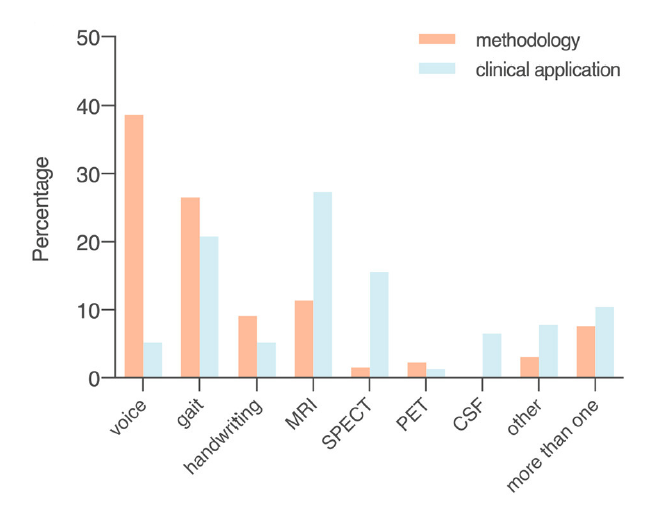
\includegraphics[width=0.5\textwidth]{./img/plot_PD_detection_methods}
	\caption{Wykres przedstawiający rozkład rodzaju danych na których bazowały systemy ML do diagnostyki PD\cite{ML_for_PD_review} (stan na dzień 14 luty 2020)}
    \label{fig:pd_detection_methods}\label{fig:figure}
\end{figure}


\subsection{Rozwiązania teoretyczne}
\label{subsec:rozwiazania-teoretyczne}

\subsection{Aplikacje rzeczywiste}
\label{subsec:aplikacje}


\subsection{Niedopatrzenia dotychczasowych rozwiązań}
\label{subsec:wady_rozwiazan}

Ostatnie badania wykazały, że możemy wytrenować dokładne modele do wykrywania oznak PD z nagrań audio.
Jednakże, istnieją rozbieżności pomiędzy badaniami i mogą być spowodowane, częściowo, przez różnice w
wykorzystywanych korpusach lub metodologii.
Dlatego w  \cite{SustainedVowelsProblems} przeprowadzono analizę, wpływu niektórych czynników na wyniki klasyfikacji.
Głównym celem artykułu była ich identyfikacja oraz stworzenie zasad, które w przyszłosći pozwolą usystematyzować
stan wiedzy w tej dziedzinie.
W badaniach skupiono się na przedłużonych samogłoskach (ang. \emph{sustained vowels}), ponieważ jak wykazano wcześniej
[...].
Przeprowadzone eksperymenty wykazały, że nieuwzględnione zmienne w metodologii, projekcie eksperymentalnym i
przygotowaniu danych prowadzą do zbyt optymistycznych wyników w badaniach nad automatyczną detekcją PD.
Czynniki, które zidentyfikowano jako przyczyniające sią do zbyt optymistycznych wyników klasyfikacji
przedstawiono na Rys. \ref{fig:factors_PD_detection} oraz omówiono poniżej.


\begin{figure}[htbp]
	\centering
	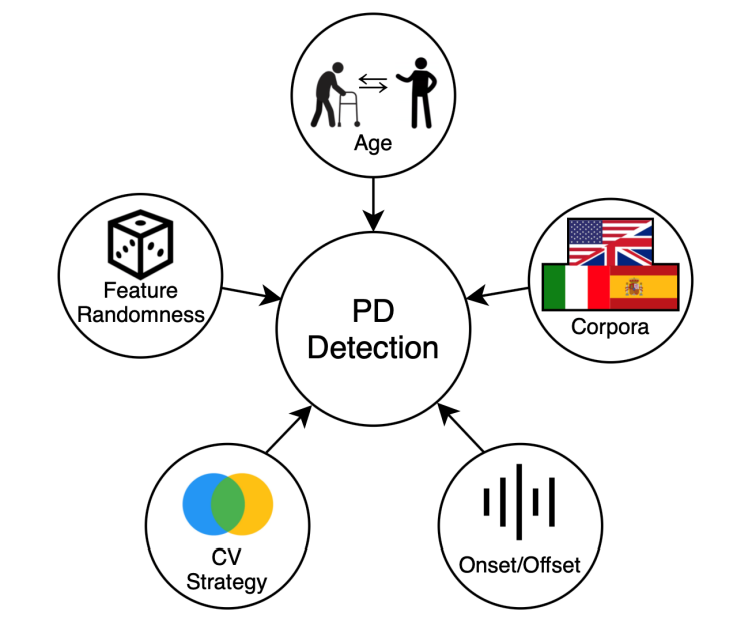
\includegraphics[width=0.4\textwidth]{./img/influence_of_factors_on_PD_detection}
	\caption{Czynniki wpływające na dokładność detekcji Parkinsona na podstawie głosu według analizy przeprowadzonej w \cite{SustainedVowelsProblems}}
    \label{fig:factors_PD_detection}
\end{figure}


\begin{enumerate}[label={\alph*)}]
	\item \textbf{Wpływ tożsamości mówcy}
	\item[] W przypadku, gdy w zbiorze danych znajduje się kilka nagrań od tego samego mówcy można postąpić na dwa sposoby.
Pierwszy z nich to podział według podmiotów (ang. \emph{subject-wise split}) polegający na tym, że nagrania od tej samej
osoby znajdują się albo w zbiorze treningowym albo testowym - nigdy w obu na raz.
W niektórych opracowań można spotkać też drugie podejście, czyli podział według rekordów (ang.\emph{record-wise split}), gdzie nagrania są losowo dzielone do zbiorów
lub intencjonalnie używa się nagrań od tej samej osoby zarówno w zbiorze testowym jak i treningowym.
Okazuje się, że podejście typu \emph{record-wise} prowadzi do wyższej dokładności niż \emph{subject-wise split}, jeśli pozostałe założenia pozostają identyczne.
Prawdopodobnie wynika to z faktu, że klasyfikator nastawia się na wykrywanie unikalnych informacji indywidualnych,
reprezentowanych przez współczynniki takie jak MFCC i PLP, a nie rzeczywiste biomarkery lub wzorce PD.
Dlatego też rekomendowana jest technika \emph{subject-wise split}, aby uniknąć zbyt optymistycznych wyników.

  	\item \textbf{Wpływ różnicy wieku między klasami}
	\item[] W literaturze można znaleźć prace wykorzystujące zbiory danych, w których  średni wiek mówców
w klasie osób chorych na PD różni się od średniego wieku w klasie osób zdrowych o ponad 5 lat.
Autorzy zapewniają o wysokiej skuteczności  swoich rozwiązań, jednak nie rozważają oni sytuacji, w której klasyfikator
uczy się wykrywać cechy powiązane z wiekiem, zamiast rzeczywistych wzorców PD.
Aby zbadać wpływ średniej różnicy wieku między dwiema klasami, w \cite{SustainedVowelsProblems} testowano różne przesunięcia rozkładu wieku.
Wraz ze wzrostem różnicy między średnim wiekiem uczestników z PD i HC, dokładność klasyfikacji konsekwentnie rosła (Rys. \ref{fig:acc_and_age_diff}).
Na tej podstawie można stwierdzić, że związany z wiekiem wpływ na głos mówców może zaburzać wyniki otrzymywane przez klasyfikator.
Dlatego też zaleca się zbilansowanie używanych zbiorów danych, tak aby średnia różnica wieku między dwoma klasami  była jak namniejsza.


\begin{figure}[htbp]
	\centering
	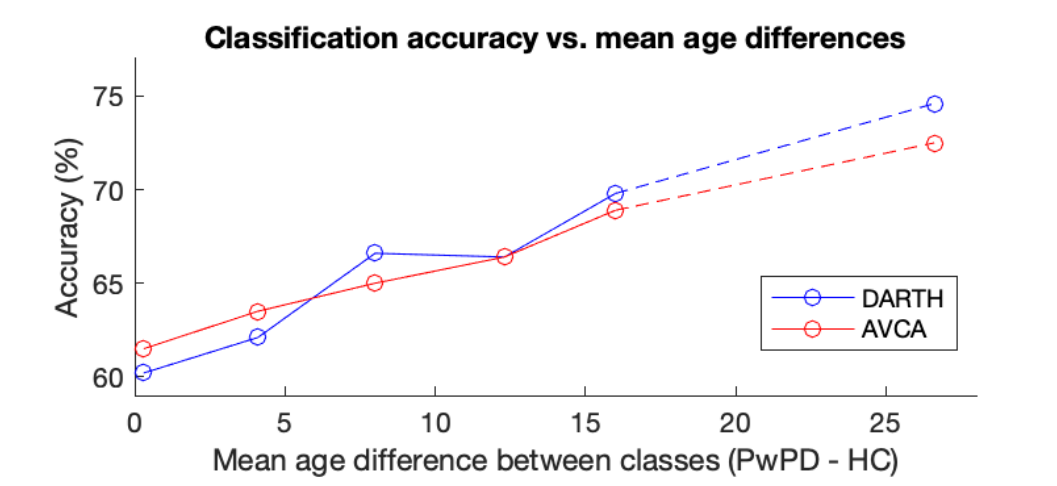
\includegraphics[width=0.7\textwidth]{./img/acc_and_age_difference}
	\caption{Wykres przedstawiający zależność różnicy wieku między klasami a dokładnością klasyfikacji \cite{SustainedVowelsProblems}}
    \label{fig:acc_and_age_diff}
\end{figure}

  	\item Wpływ losowości cech na dokładność klasyfikacji
	\item [] Im większa różnica między liczbą plików a wymiarem wektora cech, tym większe szanse na znalezienie cechy, która losowo koreluje z etykietami klas.
  	\item Łagodzenie losowego nadmiernego dopasowania przy użyciu danych programistycznych
	\item Wpływ rozpoczęcia i przesunięcia samogłosek na wyniki klasyfikacji
 	\item Eksperymenty międzykorporowe
	\item Analiza cech
\end{enumerate}



Nie są to jednak wszystkie czynniki, które zaburzają obiektywność wyników. Konieczna jest dyskusja na temat nowych
kompleksowych linii bazowych dla prowadzenia eksperymentów w automatycznym wykrywaniu PD na podstawie fonacji,
a także innych ogólnych zastosowań przetwarzania mowy.


\subsection{Wnioski}
\label{subsec:wnioski}

Prace nad automatyczną detekcją Parkinsona na podstawie głosu trwają już od dłuższego czasu.
Jednak wciąż brakuje systemu, który mógłby zostać uznany jako wystarczajaco niezawodne narzędzie diagnostyczne.
Wśród problemów, które ograniczają rzeczywiste wykorzystanie takich systemów wyróżnia się:

\begin{itemize}
\item pierwszy punkt
\item drugi punkt
\item trzeci punkt
\end{itemize}

%---------------------------------------------------------------------------
